\subsubsection{RFID}
\label{subsubsec:RFID}

Eine Funktion der Maschine ist, dass der User ohne Suchen sein Lieblingsgetränk zubereiten lassen kann. Dafür wird auf ein System zurückgegriffen, welches beispielweise auch für Zutrittskontrollen verwendet wird, RFID \footnote{Radio Frequency IDentification}.

Ein Eingrenzungskriterium für das Bauteil war, dass es es für den ausgewählten IC eine bestehende Library gibt, welche mit Arduino oder besser C kompatibel ist und dass der IC auf einem Breakot-Board erhältlich ist. Der Chip, welcher diese Anforderungen erfüllt, ist der \textbf{Mifare MFRC522}. Das Brakeout-Board ist an der Verschalung der Maschine angeschraubt.
Das Modul arbeitet auf 13.56MHz und gilt somit als kurzwelliges System (HF). \cite{nxp_semiconductors_nv_mfrc522_2017}

Das RFID-Modul ist der Reader im RFID-System. Er kann Daten vom RFID-Tag lesen. Dazu erzeugt er ein hochfrequentes, elektromagnetisches Wechselsignal mit einer Frequenz von 13.56MHz. Das Wechselfeld induziert beim Empfänger eine Spannung, welche als Energieversorgung dient. Durch Kurzschliessen der Tag-Antenne wird ein Teil der Energie des vom Reader ausgehenden Wechselfeldes verbraucht. Diese Energiedifferenz kann der Reader detektieren.

%Der Sender kann jedoch auch ein Datensignal über das Energiesignal modulieren. Die Informationen werden im Tag demoduliert und verwertet. Bei den Befehlen für den Tag geht es hauptsächlich um Lese- und Schreibmethoden. Bei einer Lesemethode des RFID wird ein Teil des Speichers abgefragt, bei Schreibmethoden wird der Speicher beschrieben. Die Reichweite für ein solches System, welches als Passivsystem deklariert ist, beträgt maximal 5cm. \cite{rfid-basisde_aufbau_2018}

\paragraph{Schema}\mbox{}

In Bild \ref{fig:Schema_RFID} ist der Schaltungsaufbau des RFID-Moduls zu sehen. Darin ersichtlich sind folgende Teilbereiche:

\begin{itemize}
\item MFRC522 RFID IC
\item Antenne
\item Anpassnetzwerk für Antenne
\item Kommunikaitonsschnittstellen
\end{itemize}

Die Schaltung ist auf dem Print mitgelayoutet. Allerdings ist das Breakout-Board die bessere Lösung, da die Bestimmung des Anpassnetzwerkes noch nicht korrekt ist und so kein Antennenkabel vom Stecker nach aussen geführt werden muss, da das verwendete Breakout-Board extern angebracht wird und die Antenne schon vorhanden ist.

\begin{figure}[H]
\center
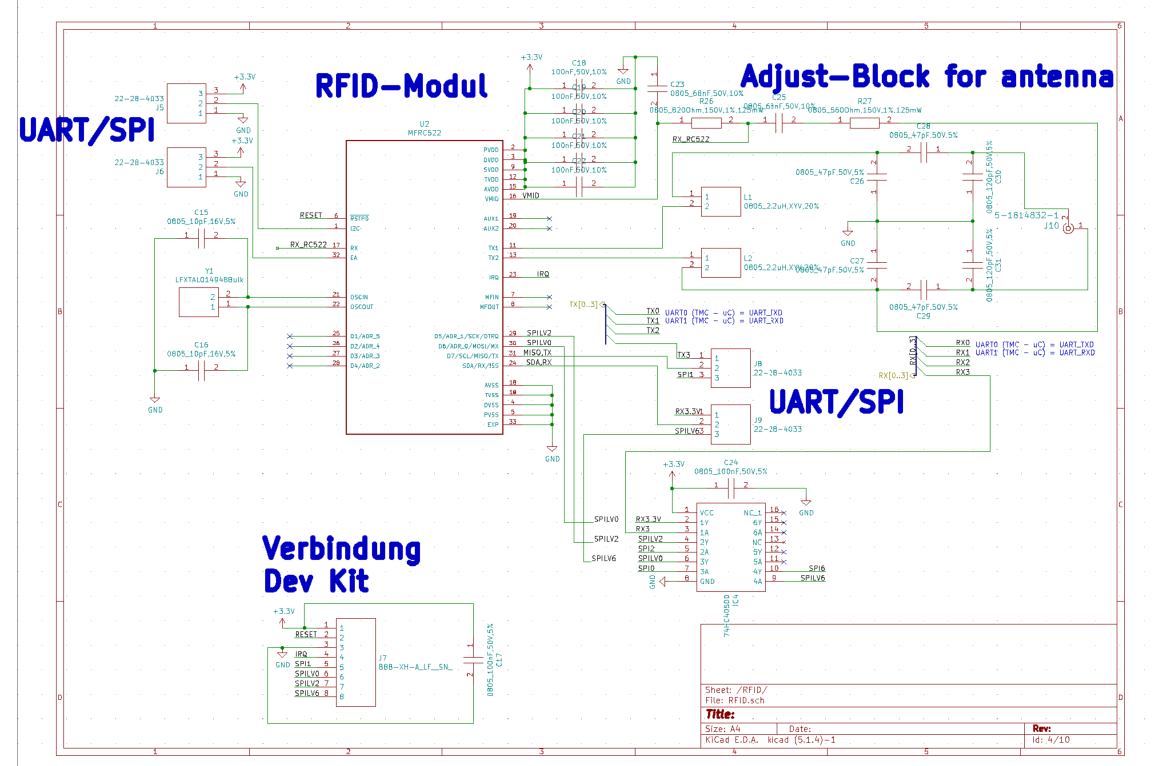
\includegraphics[width = \textwidth]{graphics/Schema_RFID}
\caption{Schema des RFID Sender/Empfänger}
\label{fig:Schema_RFID}
\end{figure}

\paragraph{Funktionsbeschrieb der Schaltung}\mbox{}

Das RFID-Modul steuert den Ablauf, damit die Datenübertragung stattfinden kann. Er verbindet die RFID-Antenne mit dem PartyMixer und schreibt bzw. liest die Informationen auf das bzw. aus dem Trägersignal. Die Herausforderung besteht im Design des Anpassnetzwerkes, welches an das IC und die Antenne angepasst werden muss. Wie die Bauteile dimensionert werden, ist in der Annotation Note 1445 von NXP Semiconductors beschrieben. Da das Breakout-Board zum Einsatz kommt, wird nicht weiter auf die Dimensionierung der Bauteile eingegangen.

Die Kommunikationsanschlüsse sind so gestaltet, dass im Falle einer zukünftigen Revision, die Kommunikation zwischen UART und SPI gewählt werden kann. Das Breakout-Board kommuniziert nur über SPI.
%In erster Linie damit keine Zeit gebraucht wird, sich mit einem Antennendesign auseinandersetzen zu müssen. Aber auch, weil der IC in ein TQFP28-Gehäuse gepackt ist, und deshalb Schwierigkeiten auftreten könnten beim Löten.